\section{Architektur des Prototypen}
Der entwickelte Prototyp ist ein Kernbestandteil dieser Arbeit. In diesem Kapitel werden die generelle Architektur, aufgetretene Herausforderungen und technische Details erläutert. Das Kapitel \hyperref[architecture]{4.2} umfasst eine technische Dokumentation des Prototypen.
\subsection{Anforderungen}
Die Anforderungen haben sich im Laufe der Entwicklung geändert und weiterentwickelt. Die Anforderungen sind im wesentlichen Architektur- und Codestil-Entscheidungen sowie Funktionsanforderungen.\\

\begin{center}
	\begin{tabularx}{0.9\linewidth}{|c|X|}
		\hline
		\multicolumn{2}{|l|}{\textbf{Technische Anforderungen}}\\
		\hline
		
		\textbf{\hyperref[tecreq1]{tec\_req1}} & Darstellen eines kompletten Absatzprozesses von Software.\\
		\hline
		
		\textbf{\hyperref[tecreq2]{tec\_req2}} & Verwendung von Carla für das darstellen des Autos.\\
		\hline
		
		\textbf{\hyperref[tecreq3]{tec\_req3}} & Einbeziehen von Uptane Architektur in die eigene.\\
		\hline
		
		\textbf{\hyperref[tecreq4]{tec\_req4}} & Monitoring \& Steuerung der Module.\\
		\hline
		
		\textbf{\hyperref[tecreq5]{tec\_req5}} & Verwenden von Android Automotive OS für die Mensch Maschine Schnittstelle.\\
		\hline
		
		\textbf{\hyperref[tecreq6]{tec\_req6}} & Bewahren einer erweiterbaren Architektur.\\
		\hline
		
		\textbf{\hyperref[tecreq7]{tec\_req7}} & Ordentliches JavaDoc\\
		\hline
		
	\end{tabularx}
\end{center}

\textbf{1. Darstellen eines kompletten Absatzprozesses von Software.}\label{tecreq1}\\
Im Rahmen der \hyperref[wsk]{Wertschöpfungskette} wurde ein \hyperref[absatzprozess]{Absatzprozess }für den behandelten \hyperref[anwendungsfall]{Anwendungsfall} ausgearbeitet. Die einzelnen Schritte sollen im Prototypen ausgewählt und durchgeführt werden können. Die einzelnen Schritte sollen in einer GUI angezeigt werden, der aktuelle Schritt soll farblich hervorgehoben werden. In einem Textfeld soll eine Beschreibung des aktuellen Schrittes stehen. Diese stellt dar, was welche Komponente in diesem Schritt tut.\\

\textbf{2. Verwendung von Carla für das darstellen des Autos.}\label{tecreq2}\\
Ein visuelles Durchlaufen des \hyperref[absatzprozess]{Absatzprozesses} soll das Verständnis des Anwendungsfalls steigern. Dazu müssen die Daten der Simulation ausgewertet werden, da die Position des Fahrzeugs maßgebend für den aktuellen Schritt ist.\\

\textbf{3. Einbeziehen von Uptane Architektur in die eigene.}\label{tecreq3}\\
Ein wichtiger Aspekt im Rahmen der Verteilung von Software ist das schaffen einer gesicherten Kommunikation zwischen Fahrzeug und Software-Server. Hierzu soll die im Forschungsseminar vorgestellte \hyperref[uptane]{Uptane Architektur} in die des Prototypen einfließen. Verschlüsselungen und weitere Details von Uptane werden nicht beachtet.\\

\textbf{4. Monitoring \& Steuerung des Absatzprozesses}\label{tecreq4}\\
Jedes Modul des Prototypen ist im Absatzprozess aktiv. Teilweise müssen Module während eines Schrittes auf die Antwort eines anderen Moduls warten, oder ein Modul verschickt eine Nachricht an ein anderes. Damit der Ablauf des Absatzprozesses verdeutlicht wird, sollen in einer GUI die aktuelle Status der Module abgebildet werden. Auch soll jedes Modul steuerbar sein, damit die Einzelentscheidungen des Prozesses veranschaulicht werden.\\

\textbf{5. Verwenden von Android Automotive OS für die Mensch Maschine Schnittstelle.}\label{tecreq5}\\
Über eine Android-Schnittstelle soll mit dem Auto interagiert werden. Hierzu wird eine Applikation bereitgestellt, über welche der Nutzer Entscheidungen bzgl. der Installation und Nutzung von Software eingeben kann.\\ 

\textbf{6. Bewahren einer erweiterbaren Architektur.}\label{tecreq6}\\
Sämtliche Module sollen das einbinden neuer Anwendungsfälle einfach handhaben können. Die Architekturen der Module soll dies unterstützen.\\

\textbf{7. Ordentliches JavaDoc}\label{tecreq7}\\
Damit der Code auch nach der Abgabe der Arbeit genutzt und erweitert werden kann, ist ein ordentliches JavaDoc zu führen.\\

\subsection{Technische Dokumentation}\label{architecture}
Nach \hyperref[tecreq3]{Anforderung Drei} soll die Uptane Architektur in die des Prototypen einbezogen werden. Diese wurde im Rahmen von Kapitel \hyperref[uptane]{2.2.1} vorgestellt und in ein erstes technisches Konzept \textit{(\hyperref[technGrundkonzept]{Kapitel 4})} eingearbeitet. Im folgenden wird die Architektur des Prototypen vorgestellt, welche ihren Ursprung aus dem zuvor erstellten Konzept zieht.\\
\begin{figure}[!h]
	\centering
	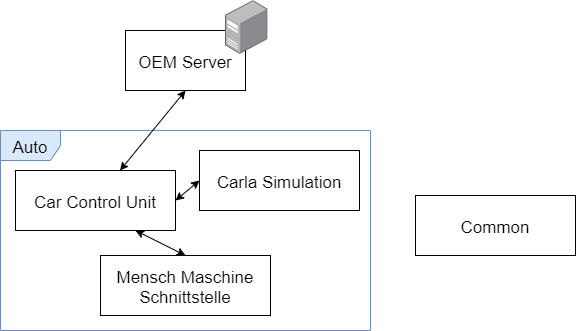
\includegraphics[width=0.8\columnwidth]{pictures/basic.png}
	\label{img:basic}
	\caption{Grundlegende Komponenten}
\end{figure}\\

Wie in Abbildung \ref{img:basic} zu sehen, umfasst der Prototyp mehrere Teilsysteme. Die Zwei wesentlichen Modulen sind der \textbf{OEM-Server} und das \textbf{Auto} \textit{(Ego-Car)}. Der OEM-Server repräsentiert die Kommunikationsinfrastruktur des Automobilherstellers und ist für das Auto die '\textbf{single source of truth}'. Das Auto wird durch die Zusammensetzung von \textbf{Mensch-Maschine-Schnittstelle} \textit{(HMI)}, \textbf{Car-Control-Unit} \textit{(CCU)} und der \textbf{Carla Simulation} dargestellt.
Die Carla Simulation beinhaltet die Darstellung eines Autos, dem 'Ego-Car', sowie der Simulation der Autoumwelt. Dieses Modul bestimmt den aktuellen Stand der Simulation, da aus der Position des Autos die möglichen Aktionen hervorgehen. Die Car-Control-Unit ist eine Kommunikations- und Steuereinheit des Autos dar und ist für die Verwaltung und Nutzung von Software zuständig. Damit eine Software auf Nutzereingaben reagieren kann, wird eine Mensch-Maschine-Schnittstelle in Form einer Android Nutzeroberfläche integriert, über welche mit dem \textbf{Auto}\textit{(blauer Kasten Abbildung \ref{img:basic})} interagiert werden kann.\\
Sämtliche Komponenten kommunizieren untereinander auf Basis der \textbf{Common Objekte}. Diese sind eine Ansammlung an Nachrichten und Objekten, welche zwischen den Komponenten verschickt werden.\\
\subsubsection{Kommunikation und Common Objekte}
\textbf{Architektur}\\
Damit die Module miteinander kommunizieren können werden Netzwerkinfrastrukturen zwischen ihnen aufgespannt \textit{(repräsentiert durch die Pfeile)}. Der OEM-Server und die CCU kommunizieren miteinander über eine Netty\footnote{QUELLE}-Verbindung. Die CCU ist mit der Carla Simulation und dem MMS jeweils über Ports verbunden. Neben diesen Netzwerkkommunikationsmethoden nutzen die Komponenten die Common-Objekten als gemeinsame Kommunikationsgrundlage. \\
\begin{figure}[!h]
	\centering
	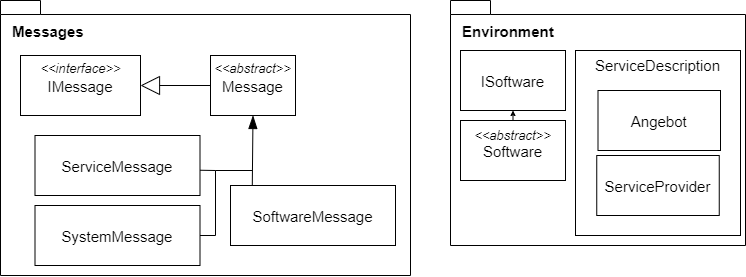
\includegraphics[width=\columnwidth]{pictures/common.png}
	\label{img:common}
	\caption{Architektur: Common Objekte}
\end{figure}\\
\textbf{Messages}\\
Das Interface \textit{IMessage} ist die oberste Klasse der Common Objekte. Sie extended java.io.Serialiable, damit die Objekte zu ByteCode umgewandelt und über die Netzwerke verschickt werden können. Die abstrakte Klasse \textit{Message }ist die Elternklasse aller folgenden Nachrichten und implementiert die Methoden \textit{IMessage}. Fort folgend wird bei allen Nachrichten zwischen \textit{Service-, Software- und SystemMessages }unterschieden. Jede dieser Klassen extended die \textit{Message}-Klasse und ist jeweils für einen wesentlichen Teil der Kommunikation zuständig.\\
\\
\textbf{Technische Dokumentation}\\
\begin{center}
	\begin{tabular}{| p{0.25\textwidth} | p{0.7\textwidth} |}
		\hline
		\textbf{Klasse} &\textbf{Beschreibung}\\
		\hline
		\textbf{ServiceMessage} &
		Jede Nachricht die im Bezug auf eine \textit{Software} verschickt wird, extended diese Klasse. In ihr wird die SoftwareID gesetzt, anhand welcher das Auto weiß auf welche Software sich die Nachricht bezieht.\\
		&
		\begin{itemize}
			\item[] \textbf{requiredSWID: String} \textit{Die ID der benötigten Software.}
			\item[] \textbf{serviceID: String} \textit{Die ID des Service Anbieters.}
		\end{itemize}\\
		\hline
		\textbf{ServiceActionMessage} \textit{extends ServiceMessage}&Die ServiceActionMessage wird von dem ServiceAnbieter\textit{(CarlaEnvironment)} an das Fahrzeug gesendet, wenn der Service genutzt werden soll. Das Fahrzeug schickt sie weiter an das CarlaCar.\\&\\
		\hline
		
	\end{tabular}
\end{center}

\textbf{Hier ist geplant:}
\begin{itemize}
	\item Jede Message beschreiben und die Assoziation zum Absatzprozess darstellen
	\item Jedes COmmonObjekt und dessen Bedeutung für den prototypen beschreiben
\end{itemize}



\subsubsection{Car-Control-Unit}
\textbf{Hier ist geplant:}
\begin{itemize}
	\item Die technische Architektur beschreiben und Lebenszyklus darstellen
	\item Bedeutung von \textbf{MessageHandler} und \textbf{SoftwareManager} verdeutlichen
	\item Auflisten: Nachrichten die von CCU verschickt bzw. empfangen werden und der Kontext der Nachrichten
	\item Herausforderungen in der implementierung
	\item ca. 4-5 Seiten
\end{itemize}

\begin{figure}[!h]
	\centering
	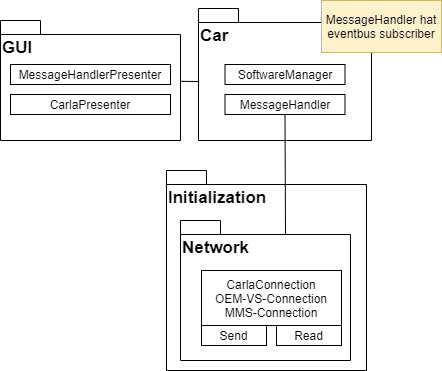
\includegraphics[width=0.8\columnwidth]{pictures/ccu.png}
	\label{img:ccu}
	\caption{Grundlegende Komponenten}
\end{figure}



\subsubsection{Software Server}\label{server}
\textbf{Hier ist geplant:}
\begin{itemize}
	\item Die technische Architektur beschreiben und Lebenszyklus darstellen
	\item Architektur im bezug auf Uptane erklären
	\item Auflisten: Nachrichten die von SwS verschickt bzw. empfangen werden und der Kontext der Nachrichten
	\item Herausforderungen in der implementierung
	\item ca. 2-3 Seiten
\end{itemize}

\begin{figure}[!h]
	\centering
	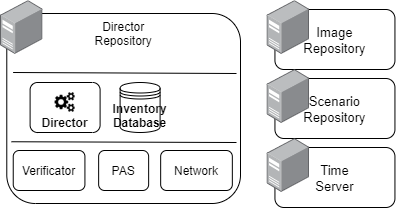
\includegraphics[width=0.8\columnwidth]{pictures/sws.png}
	\label{img:sws}
	\caption{Grundlegende Komponenten}
\end{figure}

\subsubsection{Carla}
\textbf{Hier ist geplant:}
\begin{itemize}
	\item Die technische Architektur beschreiben und Lebenszyklus darstellen
	\item Differenzieren: CarlaCar  vs. CarlaEnvironment
	\item Auflisten: Nachrichten die von Carla verschickt bzw. empfangen werden und der Kontext der Nachrichten
	\item Herausforderungen in der implementierung
	\item ca. 3-4 Seiten
\end{itemize}

\subsubsection{Mensch-Maschine-Schnittstelle}
\textbf{Hier ist geplant:}
\begin{itemize}
	\item Die technische Architektur beschreiben und Lebenszyklus darstellen
	\item Auflisten: Nachrichten die von MMS verschickt bzw. empfangen werden und der Kontext der Nachrichten
	\item ca. 2 Seiten
\end{itemize}
.
\subsection{Erweiterbarkeit und Veröffentlichung}
Dieses Kapitel kommt zum Schluss. Wird darstellen, wie der Prototyp zu erweitern ist\\
Guide: Wie füge ich eine neue SOftware + Service hinzu?